\section{Balance control}\label{sec:control}

Two controllers were implemented and tested on the nonlinear model of
\cref{sec:model}: a PID on the tilt angle and a linear-quadratic regulator
(LQR) on the full state. Both compute the total wheel torque $\tau$ once per
step of $\Delta t = \SI{5}{ms}$; the torque is held constant during the step
(\cref{sec:sim}). In this section the torque is applied without limits; the
motor model is introduced in \cref{sec:motor}.

\subsection{PID on the tilt angle}

The controller uses only $\theta$ and $\dot\theta$:
\begin{equation}
  \tau = k_p\,\theta + k_i\int_0^t \theta\,\dd t' + k_d\,\dot\theta .
  \label{eq:pid}
\end{equation}
The derivative term uses the measured $\dot\theta$ instead of a numerical
derivative of $\theta$. All gains are positive: with $\theta > 0$ the body
falls towards $+x$, and a positive torque tilts it back (\cref{eq:lin-thdd}).

\paragraph{Conditions on the gains.} With $k_i = 0$, substituting
\cref{eq:pid} in the linearised equation \cref{eq:lin-thdd} gives
\begin{equation}
  \ddot\theta = \frac{1}{D}\left[a\,\mb g l\,\theta
      - \left(a + \frac{b_0}{r}\right)\left(k_p\theta + k_d\dot\theta\right)\right]
  = \beta\,\theta - \gamma\left(k_p\theta + k_d\dot\theta\right),
  \qquad \gamma = \frac{a + b_0/r}{D} = |b_4| ,
\end{equation}
with $\beta$ and $b_4$ from \cref{eq:AB}. Rearranging,
\begin{equation}
  \ddot\theta + \gamma k_d\,\dot\theta + \left(\gamma k_p - \beta\right)\theta = 0 ,
\end{equation}
which has the form of a damped oscillator
$\ddot\theta + 2\zeta\omega_n\dot\theta + \omega_n^2\theta = 0$ with
\begin{equation}
  \omega_n^2 = \gamma k_p - \beta , \qquad \zeta = \frac{\gamma k_d}{2\omega_n} .
\end{equation}
The upright position is stable if both coefficients are positive, that is
\begin{equation}
  k_p > \frac{\beta}{\gamma} = \frac{a\,\mb g l}{a + b_0/r} = \SI{0.237}{N.m/rad},
  \qquad k_d > 0 .
\end{equation}
With $k_p = \SI{0.61}{N.m/rad}$ and $k_d = \SI{0.01}{N.m.s/rad}$:
$\omega_n = \SI{14.4}{rad/s}$ and $\zeta = 0.19$; critical damping
($\zeta = 1$) would require $k_d = 2\omega_n/\gamma = \SI{0.052}{N.m.s/rad}$.
The integral gain is $k_i = \SI{0.026}{N.m/(rad.s)}$.

\paragraph{Position.} The controller contains neither $x$ nor $\dot x$. Once
$\theta$ and $\dot\theta$ are zero, \cref{eq:pid} gives $\tau = 0$ apart from the
integral term, and by \cref{eq:lin-xdd} $\ddot x = 0$: the robot keeps the
velocity it reached while recovering. In terms of \cref{sec:lin}, the double
eigenvalue at zero associated with the position is not moved by this controller.

\subsection{Linear-quadratic regulator}

The LQR is a state feedback
\begin{equation}
  \tau = -\bm K\,\bm s , \qquad \bm K \in \mathbb R^{1\times4},
\end{equation}
whose gain minimises, for the linear model \cref{eq:lti}, the cost
\begin{equation}
  J = \int_0^\infty \left(\bm s^{\mathsf T}\bm Q\,\bm s + R\,\tau^2\right)\dd t ,
\end{equation}
where $\bm Q$ (symmetric, positive semi-definite) weights the deviation of each
state from zero and $R > 0$ weights the use of torque.

\paragraph{Gain.} Let $V(\bm s) = \bm s^{\mathsf T}\bm P\bm s$, with $\bm P$
symmetric, be the minimum cost from state $\bm s$. Optimality requires that, at
every state, the best input makes the cost rate plus the rate of change of $V$
vanish (Hamilton--Jacobi--Bellman equation):
\begin{equation}
  0 = \min_\tau\left[\bm s^{\mathsf T}\bm Q\bm s + R\tau^2
      + 2\bm s^{\mathsf T}\bm P\left(\bm A\bm s + \bm B_{\mathrm{lin}}\tau\right)\right] ,
\end{equation}
where $2\bm s^{\mathsf T}\bm P\dot{\bm s}$ is $\dd V/\dd t$. The bracket is
quadratic in $\tau$; setting its derivative to zero,
\begin{equation}
  2R\tau + 2\bm B_{\mathrm{lin}}^{\mathsf T}\bm P\bm s = 0
  \quad\Rightarrow\quad
  \tau = -R^{-1}\bm B_{\mathrm{lin}}^{\mathsf T}\bm P\,\bm s ,
  \qquad \bm K = R^{-1}\bm B_{\mathrm{lin}}^{\mathsf T}\bm P .
\end{equation}
Substituting this $\tau$ back, and writing
$2\bm s^{\mathsf T}\bm P\bm A\bm s = \bm s^{\mathsf T}(\bm A^{\mathsf T}\bm P + \bm P\bm A)\bm s$,
\begin{equation}
  0 = \bm s^{\mathsf T}\left(\bm Q + \bm A^{\mathsf T}\bm P + \bm P\bm A
      - \bm P\bm B_{\mathrm{lin}}R^{-1}\bm B_{\mathrm{lin}}^{\mathsf T}\bm P\right)\bm s
  \quad\text{for every } \bm s ,
\end{equation}
so the matrix in brackets must vanish: $\bm P$ is the solution of the
algebraic Riccati equation
\begin{equation}
  \bm A^{\mathsf T}\bm P + \bm P\bm A
  - \bm P\bm B_{\mathrm{lin}}R^{-1}\bm B_{\mathrm{lin}}^{\mathsf T}\bm P + \bm Q = \bm 0 ,
\end{equation}
computed numerically (\texttt{scipy.linalg.solve\_continuous\_are}).

\paragraph{Weights and gain.} With
$\bm Q = \operatorname{diag}(1, 10, 1, 1)$ and $R = 100$ (SI units),
\begin{equation}
  \bm K = \begin{bmatrix} -0.100 & -0.900 & -0.177 & -0.138 \end{bmatrix} .
\end{equation}
The eigenvalues of the closed-loop matrix $\bm A - \bm B_{\mathrm{lin}}\bm K$
are $-58.46$, $-3.62$ and $-1.21 \pm 0.42\,j$~\si{s^{-1}}: all have negative
real part, including the two that were at zero in \cref{sec:lin}. The gain is
designed in continuous time and applied every $\Delta t$; for the fastest
eigenvalue $|\lambda|\Delta t = 0.29$.

\subsection{Results}

Both controllers were simulated on the nonlinear model from rest with
$\theta_0 = 10^\circ$ (\cref{fig:control}).

\begin{itemize}
  \item \textbf{PID.} The tilt returns to zero within about \SI{2}{s}, with an
        oscillation consistent with $\zeta = 0.19$. The position does not
        return: $x = \SI{13.7}{cm}$ at \SI{5}{s} and \SI{18.5}{cm} at
        \SI{8}{s}, with the robot still moving at \SI{1.4}{cm/s}. Maximum
        torque: \SI{0.106}{N.m}.
  \item \textbf{LQR.} The tilt returns to zero with a single undershoot of about $2^\circ$. The robot
        moves forward by up to \SI{10.9}{cm} while recovering and then returns:
        $x = \SI{0.3}{cm}$ at \SI{5}{s}. Maximum torque: \SI{0.157}{N.m}.
\end{itemize}

\begin{figure}[h]
\centering
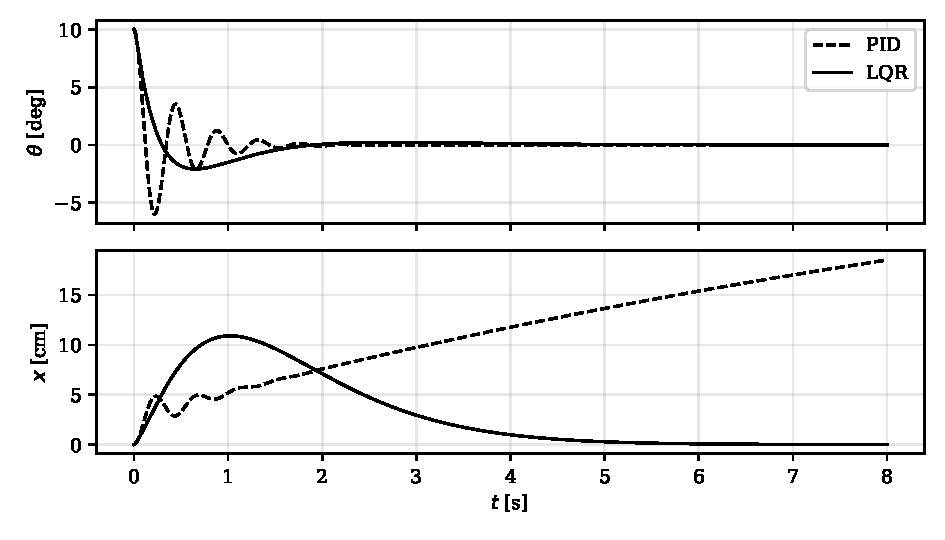
\includegraphics[width=\linewidth]{figures/control_response.pdf}
\caption{Response from rest with $\theta_0 = 10^\circ$, nonlinear model, torque
without limits. PID: $k_p = 0.61$, $k_i = 0.026$, $k_d = 0.01$. LQR:
$\bm Q = \operatorname{diag}(1,10,1,1)$, $R = 100$.}
\label{fig:control}
\end{figure}
